\documentclass[UTF8,a4paper]{ctexart}
\usepackage[utf8]{inputenc}
\usepackage{amsmath}
\usepackage{pdfpages}
\usepackage{graphicx}
\usepackage{wrapfig}
\usepackage{listings}
\usepackage{color}
\usepackage{alltt}
\usepackage{marvosym}
\usepackage{xcolor}
% Style definition file generated by highlight 3.6, http://www.andre-simon.de/ 

% Highlighting theme: Vim Editor 

\newcommand{\hlstd}[1]{\textcolor[rgb]{0,0,0}{#1}}
\newcommand{\hlnum}[1]{\textcolor[rgb]{1,0,0}{#1}}
\newcommand{\hlesc}[1]{\textcolor[rgb]{1,0.13,1}{#1}}
\newcommand{\hlstr}[1]{\textcolor[rgb]{1,0,0}{#1}}
\newcommand{\hlpps}[1]{\textcolor[rgb]{1,0,0}{#1}}
\newcommand{\hlslc}[1]{\textcolor[rgb]{0,0,1}{#1}}
\newcommand{\hlcom}[1]{\textcolor[rgb]{0,0,1}{#1}}
\newcommand{\hlppc}[1]{\textcolor[rgb]{1,0.13,1}{#1}}
\newcommand{\hlopt}[1]{\textcolor[rgb]{0,0,0}{#1}}
\newcommand{\hllin}[1]{\textcolor[rgb]{0,0,1}{#1}}
\newcommand{\hlkwa}[1]{\textcolor[rgb]{0.7,0.41,0.09}{#1}}
\newcommand{\hlkwb}[1]{\textcolor[rgb]{0,1,0}{#1}}
\newcommand{\hlkwc}[1]{\textcolor[rgb]{0.7,0.41,0.09}{#1}}
\newcommand{\hlkwd}[1]{\textcolor[rgb]{0,0,0}{#1}}
\definecolor{bgcolor}{rgb}{1,1,1}


\title{计算机原理第三次实验报告}
\author{张蔚桐\ 2015011493\ 自55}
\begin {document}
\maketitle
\section{实验目的}
\begin{enumerate}
\item 练习使用子程序和宏
\item 练习使用功能调用(INT 21H)中关于字符输入及字符输出的部分
\end{enumerate}
\section{实验内容}
实验完成了所有的必做和选做任务,下面按照程序执行的流程分块解释。

程序事先存储若干字符串方便后期显示的时候调用,同时将数据存储在1000H的偏移地址上。

程序开始执行后,首先完成必要的幅值工作和初始化工作,之后在Line30开始输出字符串“INPUT 10 DECIMAL NUMBER:”提示用户输入十个十进制数,Line33时,程序将DI指针移向输入内存块NUMBERS的最后一个单元,之后进入循环输入

整个循环退出的条件是DI指针移动到NUMBERS偏移地址之前,这样完成了对NUMBERS数据区的写入操作

在循环体内执行如下操作

首先调用INT 21H中断完成一个字符的读入工作,调用模式为(AH=08H)即输入不回显,检查输入的字符,如果为0DH(回车)的话更换为空格重新输出,保证输入格式的美观性,到此完成Line44之前的工作

之后开始对输入的字符进行检查,如Line47开始,首先检查是否为ASCII码的数字,如果为数字的话所执行的语句在Line53所示,检查DH(已经输入的数字)是否超过两位,如果超过两位,跳转到OVER处理块

如果输入正常,则左移DH4位,将DL从ASCII码转换为数字,之后将DL加到DH上,完成对DH的修改

如果输入的字符不是数字,如Line48等行所示,将跳转至NOTNUM处理块

下面叙述NOTNUM处理块的行为,首先检测输入的字符是否为空格,如果输入的字符为回车,因为已经在上面所述的步骤中进行了替换,因此可以一起处理。如果此时DH非零,说明结束了一个数字的输入,进入后续的OUTPUT处理块,否则返回循环开始,重新输入,相当于连续输入多个空格(回车)是无效行为

如果输入的非数字不是空格(或回车)的话,说明输入了错误字符,如Line64所示,程序显示错误原因“NOT DECIMAL NUMBER!”并通过调用CORRECT函数,显示当前的错误信息

现在说明OVER处理块的处理形式,和上面一样,具体的实现如Line69所示,程序显示错误原因“TOO MANY DIGITS”,并通过调用CORRECT函数,显示当前的错误信息

下面说明CORRECT函数的处理方式,具体实现Line137所示,首先程序调用SHOW函数显示当前已经输入的数字,其次程序提示用户还需要输入的数字,如Line147所示,首先程序将DI和数据域NUMBERS开始的地址的差赋给DX,则DL便是所要求的还需要输入的数字个数,接下来对DL的值进行分析,如果DL==10,则直接调用已经写好的数据域AUX输出10,否则DL加030H并利用INT 21H的AH=02H模式输出字符,在此前后,程序显示一些交互的信息,具体方式可见Line138之后的具体实现,主要方式是调用INT 21H的AH=09H的中断,具体叙述略去

下面简述SHOW函数的具体实现,首先仍然使用INT 21H的AH=09H中断进行一些用户交互信息的输出,之后程序将SI置为NUMBERS区尾地址,并逐字节读取直到DI==SI,在每次读取到DL后,拷贝到DH,其中DH去低4位,DL取高4位,分别移到相对应的低4位补加030H转ASCII码,先高位DL后低位DH调用INT 21H的AH=02H输出字符,之后程序依然完成一些用户交互上而定输出。其中具体实现见Line160

下面简述循环中最后一个模块OUTPUT的实现,首先将DH中的值移到DI所指示的内存中,递减DI,清空DH,等待下次输入,具体实现在Line78

至此,程序完成输入部分的操作

在Line84,程序开始调用WHOLE函数逐个显示输入的数值,WHOLE显示一个BX中信息,因此首先这里显示MESSAGE中的用户交互信息,WHOLE的具体实现在Line185,具体的方式和之前提到的SHOW大同小异,这里就不进行进一步的叙述了,唯一的不同是,输出的间隔从空格改变成为了换行符

在Line90程序开始执行冒泡排序,具体算法如下

首先程序将DL标志置零,在遍历中一旦发现有前面的字符大于后面的字符的情况,DL变为1,程序在Line101退出直到DL为0,说明整个数组已经从小到大排序,在遍历中,程序执行如下操作

内层循环开始时,程序将DI指向NUMBERS开始地址,并读取两位到AX,其中AL是前一位,AH是后一位,一旦AL大于AH,则将AL和AH交换顺序,重新将AX写入原位置,完成了检查和交换,之后DI递增,对于10个数的数组,程序执行9次。具体在Line94附近实现

在完成了冒泡排序后,数组从前到后是从小到大的排列,再次调用WHOLE函数,从后向前输出数组中的元素,完成排序

同时,直接输出数组的最后的一个元素,完成最大数的输出工作

至此,程序完成要求的所有工作,当然在上面执行的过程中,存在着一些利用INT 21H,主要是AH=09H的输出用户交互的工作

程序在Line131行将通过INT 21H,AH=04CH将控制权转回系统,并返回AL=0,之前所述的操作在前面几行进行

程序的代码如下所示,运行时的截图如图\ref{1},\ref{2}所示\\


\documentclass{article}
\usepackage{color}
\usepackage{alltt}
\usepackage{marvosym}

% Style definition file generated by highlight 3.6, http://www.andre-simon.de/ 

% Highlighting theme: Vim Editor 

\newcommand{\hlstd}[1]{\textcolor[rgb]{0,0,0}{#1}}
\newcommand{\hlnum}[1]{\textcolor[rgb]{1,0,0}{#1}}
\newcommand{\hlesc}[1]{\textcolor[rgb]{1,0.13,1}{#1}}
\newcommand{\hlstr}[1]{\textcolor[rgb]{1,0,0}{#1}}
\newcommand{\hlpps}[1]{\textcolor[rgb]{1,0,0}{#1}}
\newcommand{\hlslc}[1]{\textcolor[rgb]{0,0,1}{#1}}
\newcommand{\hlcom}[1]{\textcolor[rgb]{0,0,1}{#1}}
\newcommand{\hlppc}[1]{\textcolor[rgb]{1,0.13,1}{#1}}
\newcommand{\hlopt}[1]{\textcolor[rgb]{0,0,0}{#1}}
\newcommand{\hllin}[1]{\textcolor[rgb]{0,0,1}{#1}}
\newcommand{\hlkwa}[1]{\textcolor[rgb]{0.7,0.41,0.09}{#1}}
\newcommand{\hlkwb}[1]{\textcolor[rgb]{0,1,0}{#1}}
\newcommand{\hlkwc}[1]{\textcolor[rgb]{0.7,0.41,0.09}{#1}}
\newcommand{\hlkwd}[1]{\textcolor[rgb]{0,0,0}{#1}}
\definecolor{bgcolor}{rgb}{1,1,1}



\title{prog.asm}
\begin{document}
\pagecolor{bgcolor}
\noindent
\ttfamily
\hlstd{\hllin{01\ }DATA\ }\hlkwa{SEGMENT}\\
\hllin{02\ }\hlstd{MESSAGE0\ }\hlkwa{DB\ }\hlstd{}\hlstr{'INPUT\ 10\ DECIMAL\ NUMBER:'}\hlstd{}\hlopt{,}\hlstd{}\hlnum{0}\hlstd{}\hlkwb{DH}\hlstd{}\hlopt{,}\hlstd{}\hlnum{0}\hlstd{}\hlkwb{AH}\hlstd{}\hlopt{,}\hlstd{}\hlstr{'\$'}\hlstd{\\
\hllin{03\ }MESSAGE1\ }\hlkwa{DB\ }\hlstd{}\hlstr{'YOU\ HAVE\ INPUT:\ '}\hlstd{}\hlopt{,}\hlstd{}\hlstr{'\$'}\hlstd{\\
\hllin{04\ }MESSAGE2\ }\hlkwa{DB\ }\hlstd{}\hlnum{0}\hlstd{}\hlkwb{DH}\hlstd{}\hlopt{,}\hlstd{}\hlnum{0}\hlstd{}\hlkwb{AH}\hlstd{}\hlopt{,}\hlstd{}\hlstr{'YOU\ HAVE\ TO\ INPUT\ ANOTHER\ \$'}\hlstd{\\
\hllin{05\ }MESSAGE3\ }\hlkwa{DB\ }\hlstd{}\hlstr{'\ NUMBERS.'}\hlstd{}\hlopt{,}\hlstd{}\hlnum{0}\hlstd{}\hlkwb{DH}\hlstd{}\hlopt{,}\hlstd{}\hlnum{0}\hlstd{}\hlkwb{AH}\hlstd{}\hlopt{,}\hlstd{}\hlstr{'\$'}\hlstd{\\
\hllin{06\ }ERROR1\ }\hlkwa{DB\ }\hlstd{}\hlnum{0}\hlstd{}\hlkwb{DH}\hlstd{}\hlopt{,}\hlstd{}\hlnum{0}\hlstd{}\hlkwb{AH}\hlstd{}\hlopt{,}\hlstd{}\hlstr{'NOT\ DECIMAL\ NUMBER!'}\hlstd{}\hlopt{,}\hlstd{}\hlnum{0}\hlstd{}\hlkwb{DH}\hlstd{}\hlopt{,}\hlstd{}\hlnum{0}\hlstd{}\hlkwb{AH}\hlstd{}\hlopt{,}\hlstd{}\hlstr{'\$'}\hlstd{\\
\hllin{07\ }ERROR2\ }\hlkwa{DB\ }\hlstd{}\hlnum{0}\hlstd{}\hlkwb{DH}\hlstd{}\hlopt{,}\hlstd{}\hlnum{0}\hlstd{}\hlkwb{AH}\hlstd{}\hlopt{,}\hlstd{}\hlstr{'TOO\ MANY\ DIGITS'}\hlstd{}\hlopt{,}\hlstd{}\hlnum{0}\hlstd{}\hlkwb{DH}\hlstd{}\hlopt{,}\hlstd{}\hlnum{0}\hlstd{}\hlkwb{AH}\hlstd{}\hlopt{,}\hlstd{}\hlstr{'\$'}\hlstd{\\
\hllin{08\ }SORT\ }\hlkwa{DB\ }\hlstd{}\hlstr{'$>$$>$$>$\ AFTER\ SORTED\ $<$$<$$<$'}\hlstd{}\hlopt{,}\hlstd{}\hlnum{0}\hlstd{}\hlkwb{DH}\hlstd{}\hlopt{,}\hlstd{}\hlnum{0}\hlstd{}\hlkwb{AH}\hlstd{}\hlopt{,}\hlstd{}\hlstr{'\$'}\hlstd{\\
\hllin{09\ }MAX\ }\hlkwa{DB\ }\hlstd{}\hlstr{'$>$$>$$>$\ MAX\ NUMBER:\ '}\hlstd{}\hlopt{,}\hlstd{}\hlstr{'\$'}\hlstd{\\
\hllin{10\ }AUX\ }\hlkwa{DB\ }\hlstd{}\hlstr{'10'}\hlstd{}\hlopt{,}\hlstd{}\hlstr{'\$'}\hlstd{}\\
\hllin{11\ }\hlkwa{ORG\ }\hlstd{}\hlnum{1000H}\\
\hllin{12\ }\hlstd{NUMBERS\ }\hlkwa{DB\ }\hlstd{}\hlnum{10\ }\hlstd{DUP}\hlopt{(}\hlstd{?}\hlopt{)\ }\\
\hllin{13\ }\hlstd{DATA\ }\hlkwa{ENDS}\\
\hllin{14\ }\hlstd{\\
\hllin{15\ }STACK\ }\hlkwa{SEGMENT\ }\hlstd{PARA\ STACK}\\
\hllin{16\ }\hlkwa{DB\ }\hlstd{}\hlnum{10\ }\hlstd{DUP}\hlopt{(}\hlstd{?}\hlopt{)}\\
\hllin{17\ }\hlstd{STACK\ }\hlkwa{ENDS}\\
\hllin{18\ }\hlstd{\\
\hllin{19\ }CODE\ }\hlkwa{SEGMENT\ }\\
\hllin{20\ }\hlstd{}\hlkwa{ASSUME\ }\hlstd{}\hlkwb{ES}\hlstd{}\hlopt{:}\hlstd{DATA}\hlopt{,}\hlstd{}\hlkwb{DS}\hlstd{}\hlopt{:}\hlstd{DATA}\hlopt{,}\hlstd{}\hlkwb{CS}\hlstd{}\hlopt{:}\hlstd{CODE}\hlopt{,}\hlstd{}\hlkwb{SS}\hlstd{}\hlopt{:}\hlstd{STACK}\\
\hllin{21\ }\hlkwc{START:}\\
\hllin{22\ }\hlstd{}\hlkwa{MOV\ }\hlstd{}\hlkwb{AX}\hlstd{}\hlopt{,}\hlstd{DATA}\\
\hllin{23\ }\hlkwa{MOV\ }\hlstd{}\hlkwb{ES}\hlstd{}\hlopt{,}\hlstd{}\hlkwb{AX}\\
\hllin{24\ }\hlstd{}\hlkwa{MOV\ }\hlstd{}\hlkwb{DS}\hlstd{}\hlopt{,}\hlstd{}\hlkwb{AX}\\
\hllin{25\ }\hlstd{}\hlkwa{MOV\ }\hlstd{}\hlkwb{AX}\hlstd{}\hlopt{,}\hlstd{STACK}\\
\hllin{26\ }\hlkwa{MOV\ }\hlstd{}\hlkwb{SS}\hlstd{}\hlopt{,}\hlstd{}\hlkwb{AX}\\
\hllin{27\ }\hlstd{}\hlkwa{LEA\ }\hlstd{}\hlkwb{DI}\hlstd{}\hlopt{,}\hlstd{NUMBERS}\\
\hllin{28\ }\hlkwa{MOV\ }\hlstd{}\hlkwb{CL}\hlstd{}\hlopt{,}\hlstd{}\hlnum{4}\\
\hllin{29\ }\hlstd{}\hlslc{;READ\ IN\ 10\ NUMBERS}\\
\hllin{30\ }\hlstd{}\hlkwa{MOV\ }\hlstd{}\hlkwb{DX}\hlstd{}\hlopt{,}\hlstd{}\hlkwb{OFFSET\ }\hlstd{MESSAGE0}\\
\hllin{31\ }\hlkwa{MOV\ }\hlstd{}\hlkwb{AH}\hlstd{}\hlopt{,}\hlstd{}\hlnum{09H}\\
\hllin{32\ }\hlstd{}\hlkwa{INT\ }\hlstd{}\hlnum{21H}\\
\hllin{33\ }\hlstd{}\hlkwa{ADD\ }\hlstd{}\hlkwb{DI}\hlstd{}\hlopt{,}\hlstd{}\hlnum{09H}\\
\hllin{34\ }\hlstd{}\hlkwc{L1:}\\
\hllin{35\ }\hlstd{\ }\hlslc{;IO\ AND\ REFINE\ THE\ FORMAT}\\
\hllin{36\ }\hlstd{\ }\hlkwa{MOV\ }\hlstd{}\hlkwb{AH}\hlstd{}\hlopt{,}\hlstd{}\hlnum{08H}\\
\hllin{37\ }\hlstd{\ }\hlkwa{INT\ }\hlstd{}\hlnum{21H}\\
\hllin{38\ }\hlstd{\ }\hlkwa{MOV\ }\hlstd{}\hlkwb{DL}\hlstd{}\hlopt{,}\hlstd{}\hlkwb{AL}\\
\hllin{39\ }\hlstd{\ }\hlkwa{CMP\ }\hlstd{}\hlkwb{DL}\hlstd{}\hlopt{,}\hlstd{}\hlnum{0}\hlstd{}\hlkwb{DH}\\
\hllin{40\ }\hlstd{\ }\hlkwa{JNE\ }\hlstd{L2\\
\hllin{41\ }\ }\hlkwa{MOV\ }\hlstd{}\hlkwb{DL}\hlstd{}\hlopt{,}\hlstd{}\hlstr{'\ '}\hlstd{\\
\hllin{42\ }\ L2}\hlopt{:}\\
\hllin{43\ }\hlstd{\ }\hlkwa{MOV\ }\hlstd{}\hlkwb{AH}\hlstd{}\hlopt{,}\hlstd{}\hlnum{02H}\\
\hllin{44\ }\hlstd{\ }\hlkwa{INT\ }\hlstd{}\hlnum{21H}\\
\hllin{45\ }\hlstd{\ }\hlslc{;WORD\ IN\ DL}\\
\hllin{46\ }\hlstd{\ }\hlslc{;SET\ THE\ WORD\ IN\ DH}\\
\hllin{47\ }\hlstd{\ }\hlkwa{CMP\ }\hlstd{}\hlkwb{DL}\hlstd{}\hlopt{,}\hlstd{}\hlnum{030H}\\
\hllin{48\ }\hlstd{\ }\hlkwa{JB\ }\hlstd{NOTNUM\\
\hllin{49\ }\ }\hlkwa{CMP\ }\hlstd{}\hlkwb{DL}\hlstd{}\hlopt{,}\hlstd{}\hlnum{039H}\\
\hllin{50\ }\hlstd{\ }\hlkwa{JA\ }\hlstd{NOTNUM\\
\hllin{51\ }\ }\hlslc{;NOW\ THE\ INPUT\ SHOULD\ BE\ A\ NUMBER}\\
\hllin{52\ }\hlstd{\ }\hlslc{;CHECK\ THE\ DH}\\
\hllin{53\ }\hlstd{\ }\hlkwa{CMP\ }\hlstd{}\hlkwb{DH}\hlstd{}\hlopt{,}\hlstd{}\hlnum{00}\hlstd{FH\\
\hllin{54\ }\ }\hlkwa{JA\ }\hlstd{OVER\\
\hllin{55\ }\ }\hlslc{;NOW\ EVERYTHING\ OK}\\
\hllin{56\ }\hlstd{\ }\hlkwa{AND\ }\hlstd{}\hlkwb{DL}\hlstd{}\hlopt{,}\hlstd{}\hlnum{00}\hlstd{FH\\
\hllin{57\ }\ }\hlkwa{SHL\ }\hlstd{}\hlkwb{DH}\hlstd{}\hlopt{,}\hlstd{}\hlkwb{CL}\\
\hllin{58\ }\hlstd{\ }\hlkwa{ADD\ }\hlstd{}\hlkwb{DH}\hlstd{}\hlopt{,}\hlstd{}\hlkwb{DL}\\
\hllin{59\ }\hlstd{\ }\hlkwa{JMP\ }\hlstd{L1\\
\hllin{60\ }\ NOTNUM}\hlopt{:}\\
\hllin{61\ }\hlstd{}\hlstd{\ \ }\hlstd{}\hlslc{;CHECK\ THE\ '\ '\ }\\
\hllin{62\ }\hlstd{}\hlstd{\ \ }\hlstd{}\hlkwa{CMP\ }\hlstd{}\hlkwb{DL}\hlstd{}\hlopt{,}\hlstd{}\hlstr{'\ '}\hlstd{\\
\hllin{63\ }}\hlstd{\ \ }\hlstd{}\hlkwa{JE\ }\hlstd{L3\\
\hllin{64\ }}\hlstd{\ \ }\hlstd{}\hlkwa{MOV\ }\hlstd{}\hlkwb{DX}\hlstd{}\hlopt{,}\hlstd{}\hlkwb{OFFSET\ }\hlstd{ERROR1\\
\hllin{65\ }}\hlstd{\ \ }\hlstd{}\hlkwa{MOV\ }\hlstd{}\hlkwb{AH}\hlstd{}\hlopt{,}\hlstd{}\hlnum{09H}\\
\hllin{66\ }\hlstd{}\hlstd{\ \ }\hlstd{}\hlkwa{INT\ }\hlstd{}\hlnum{21H}\\
\hllin{67\ }\hlstd{}\hlstd{\ \ }\hlstd{}\hlkwa{JMP\ }\hlstd{L6\\
\hllin{68\ }\ OVER}\hlopt{:}\\
\hllin{69\ }\hlstd{}\hlstd{\ \ }\hlstd{}\hlkwa{MOV\ }\hlstd{}\hlkwb{DX}\hlstd{}\hlopt{,}\hlstd{}\hlkwb{OFFSET\ }\hlstd{ERROR2\\
\hllin{70\ }}\hlstd{\ \ }\hlstd{}\hlkwa{MOV\ }\hlstd{}\hlkwb{AH}\hlstd{}\hlopt{,}\hlstd{}\hlnum{09H}\\
\hllin{71\ }\hlstd{}\hlstd{\ \ }\hlstd{}\hlkwa{INT\ }\hlstd{}\hlnum{21H}\\
\hllin{72\ }\hlstd{}\hlstd{\ \ }\hlstd{L6}\hlopt{:}\\
\hllin{73\ }\hlstd{}\hlstd{\ \ }\hlstd{}\hlkwa{CALL\ }\hlstd{CORRECT\\
\hllin{74\ }}\hlstd{\ \ }\hlstd{}\hlkwa{JMP\ }\hlstd{L1\\
\hllin{75\ }\ L3}\hlopt{:}\\
\hllin{76\ }\hlstd{\ }\hlkwa{CMP\ }\hlstd{}\hlkwb{DH}\hlstd{}\hlopt{,}\hlstd{}\hlnum{0}\\
\hllin{77\ }\hlstd{\ }\hlkwa{JE\ }\hlstd{L1\\
\hllin{78\ }\ OUTPUT}\hlopt{:}\\
\hllin{79\ }\hlstd{\ }\hlkwa{MOV\ }\hlstd{}\hlkwb{BYTE\ PTR\ }\hlstd{}\hlopt{{[}}\hlstd{}\hlkwb{DI}\hlstd{}\hlopt{{]},}\hlstd{}\hlkwb{DH}\\
\hllin{80\ }\hlstd{\ }\hlkwa{DEC\ }\hlstd{}\hlkwb{DI}\\
\hllin{81\ }\hlstd{\ }\hlkwa{MOV\ }\hlstd{}\hlkwb{DH}\hlstd{}\hlopt{,}\hlstd{}\hlnum{0}\\
\hllin{82\ }\hlstd{\ }\hlkwa{CMP\ }\hlstd{}\hlkwb{DI}\hlstd{}\hlopt{,}\hlstd{}\hlkwb{OFFSET\ }\hlstd{NUMBERS}\\
\hllin{83\ }\hlkwa{JNB\ }\hlstd{L1}\\
\hllin{84\ }\hlkwa{MOV\ }\hlstd{}\hlkwb{BX}\hlstd{}\hlopt{,}\hlstd{}\hlkwb{OFFSET\ }\hlstd{MESSAGE1}\\
\hllin{85\ }\hlkwa{CALL\ }\hlstd{WHOLE}\\
\hllin{86\ }\hlkwc{L11:}\\
\hllin{87\ }\hlstd{\ }\hlkwa{MOV\ }\hlstd{}\hlkwb{DL}\hlstd{}\hlopt{,}\hlstd{}\hlnum{0}\\
\hllin{88\ }\hlstd{\ }\hlkwa{MOV\ }\hlstd{}\hlkwb{CX}\hlstd{}\hlopt{,}\hlstd{}\hlnum{9}\\
\hllin{89\ }\hlstd{\ }\hlkwa{LEA\ }\hlstd{}\hlkwb{DI}\hlstd{}\hlopt{,}\hlstd{NUMBERS\\
\hllin{90\ }\ L12}\hlopt{:}\\
\hllin{91\ }\hlstd{}\hlstd{\ \ }\hlstd{}\hlkwa{MOV\ }\hlstd{}\hlkwb{AX}\hlstd{}\hlopt{,{[}}\hlstd{}\hlkwb{DI}\hlstd{}\hlopt{{]}}\\
\hllin{92\ }\hlstd{}\hlstd{\ \ }\hlstd{}\hlkwa{CMP\ }\hlstd{}\hlkwb{AL}\hlstd{}\hlopt{,}\hlstd{}\hlkwb{AH}\\
\hllin{93\ }\hlstd{}\hlstd{\ \ }\hlstd{}\hlkwa{JNA\ }\hlstd{NORM\\
\hllin{94\ }}\hlstd{\ \ }\hlstd{}\hlkwa{MOV\ }\hlstd{}\hlkwb{DL}\hlstd{}\hlopt{,}\hlstd{}\hlnum{1}\\
\hllin{95\ }\hlstd{}\hlstd{\ \ }\hlstd{}\hlkwa{XCHG\ }\hlstd{}\hlkwb{AL}\hlstd{}\hlopt{,}\hlstd{}\hlkwb{AH}\\
\hllin{96\ }\hlstd{}\hlstd{\ \ }\hlstd{}\hlkwa{MOV\ }\hlstd{}\hlopt{{[}}\hlstd{}\hlkwb{DI}\hlstd{}\hlopt{{]},}\hlstd{}\hlkwb{AX}\\
\hllin{97\ }\hlstd{}\hlstd{\ \ }\hlstd{NORM}\hlopt{:}\\
\hllin{98\ }\hlstd{}\hlstd{\ \ }\hlstd{}\hlkwa{INC\ }\hlstd{}\hlkwb{DI}\\
\hllin{99\ }\hlstd{}\hlstd{\ \ }\hlstd{}\hlkwa{LOOP\ }\hlstd{L12\\
\hllin{100\ }\ }\hlkwa{CMP\ }\hlstd{}\hlkwb{DL}\hlstd{}\hlopt{,}\hlstd{}\hlnum{0}\\
\hllin{101\ }\hlstd{}\hlkwa{JNE\ }\hlstd{L11}\\
\hllin{102\ }\hlkwa{MOV\ }\hlstd{}\hlkwb{CL}\hlstd{}\hlopt{,}\hlstd{}\hlnum{4}\\
\hllin{103\ }\hlstd{}\hlkwa{MOV\ }\hlstd{}\hlkwb{AH}\hlstd{}\hlopt{,}\hlstd{}\hlnum{02H}\\
\hllin{104\ }\hlstd{}\hlkwa{MOV\ }\hlstd{}\hlkwb{DL}\hlstd{}\hlopt{,}\hlstd{}\hlnum{0}\hlstd{}\hlkwb{DH}\\
\hllin{105\ }\hlstd{}\hlkwa{INT\ }\hlstd{}\hlnum{21H}\\
\hllin{106\ }\hlstd{}\hlkwa{MOV\ }\hlstd{}\hlkwb{DL}\hlstd{}\hlopt{,}\hlstd{}\hlnum{0}\hlstd{}\hlkwb{AH}\\
\hllin{107\ }\hlstd{}\hlkwa{INT\ }\hlstd{}\hlnum{21H}\\
\hllin{108\ }\hlstd{}\hlkwa{MOV\ }\hlstd{}\hlkwb{DX}\hlstd{}\hlopt{,}\hlstd{}\hlkwb{OFFSET\ }\hlstd{MAX}\\
\hllin{109\ }\hlkwa{MOV\ }\hlstd{}\hlkwb{AH}\hlstd{}\hlopt{,}\hlstd{}\hlnum{09H}\\
\hllin{110\ }\hlstd{}\hlkwa{INT\ }\hlstd{}\hlnum{21H}\\
\hllin{111\ }\hlstd{}\hlkwa{MOV\ }\hlstd{}\hlkwb{AH}\hlstd{}\hlopt{,}\hlstd{}\hlnum{02H}\\
\hllin{112\ }\hlstd{}\hlkwa{LEA\ }\hlstd{}\hlkwb{SI}\hlstd{}\hlopt{,}\hlstd{NUMBERS}\\
\hllin{113\ }\hlkwa{ADD\ }\hlstd{}\hlkwb{SI}\hlstd{}\hlopt{,}\hlstd{}\hlnum{09H}\\
\hllin{114\ }\hlstd{}\hlkwa{MOV\ }\hlstd{}\hlkwb{AH}\hlstd{}\hlopt{,}\hlstd{}\hlnum{02H}\\
\hllin{115\ }\hlstd{}\hlkwa{MOV\ }\hlstd{}\hlkwb{DL}\hlstd{}\hlopt{,}\hlstd{}\hlkwb{BYTE\ PTR\ }\hlstd{}\hlopt{{[}}\hlstd{}\hlkwb{SI}\hlstd{}\hlopt{{]}}\\
\hllin{116\ }\hlstd{}\hlkwa{MOV\ }\hlstd{}\hlkwb{DH}\hlstd{}\hlopt{,}\hlstd{}\hlkwb{DL}\\
\hllin{117\ }\hlstd{}\hlkwa{SHR\ }\hlstd{}\hlkwb{DL}\hlstd{}\hlopt{,}\hlstd{}\hlkwb{CL}\\
\hllin{118\ }\hlstd{}\hlkwa{JZ\ }\hlstd{L13}\\
\hllin{119\ }\hlkwa{ADD\ }\hlstd{}\hlkwb{DL}\hlstd{}\hlopt{,}\hlstd{}\hlnum{030H}\\
\hllin{120\ }\hlstd{}\hlkwa{INT\ }\hlstd{}\hlnum{21H}\\
\hllin{121\ }\hlstd{}\hlkwc{L13:}\\
\hllin{122\ }\hlstd{}\hlkwa{AND\ }\hlstd{}\hlkwb{DH}\hlstd{}\hlopt{,}\hlstd{}\hlnum{00}\hlstd{FH}\\
\hllin{123\ }\hlkwa{ADD\ }\hlstd{}\hlkwb{DH}\hlstd{}\hlopt{,}\hlstd{}\hlnum{030H}\\
\hllin{124\ }\hlstd{}\hlkwa{MOV\ }\hlstd{}\hlkwb{DL}\hlstd{}\hlopt{,}\hlstd{}\hlkwb{DH}\\
\hllin{125\ }\hlstd{}\hlkwa{INT\ }\hlstd{}\hlnum{21H}\\
\hllin{126\ }\hlstd{}\hlkwa{MOV\ }\hlstd{}\hlkwb{DL}\hlstd{}\hlopt{,}\hlstd{}\hlnum{0}\hlstd{}\hlkwb{DH}\\
\hllin{127\ }\hlstd{}\hlkwa{INT\ }\hlstd{}\hlnum{21H}\\
\hllin{128\ }\hlstd{}\hlkwa{MOV\ }\hlstd{}\hlkwb{DL}\hlstd{}\hlopt{,}\hlstd{}\hlnum{0}\hlstd{}\hlkwb{AH}\\
\hllin{129\ }\hlstd{}\hlkwa{INT\ }\hlstd{}\hlnum{21H}\\
\hllin{130\ }\hlstd{}\\
\hllin{131\ }\hlkwa{MOV\ }\hlstd{}\hlkwb{BX}\hlstd{}\hlopt{,}\hlstd{}\hlkwb{OFFSET\ }\hlstd{SORT}\\
\hllin{132\ }\hlkwa{CALL\ }\hlstd{WHOLE}\\
\hllin{133\ }\hlkwa{MOV\ }\hlstd{}\hlkwb{AL}\hlstd{}\hlopt{,}\hlstd{}\hlnum{0}\\
\hllin{134\ }\hlstd{}\hlkwa{MOV\ }\hlstd{}\hlkwb{AH}\hlstd{}\hlopt{,}\hlstd{}\hlnum{04}\hlstd{}\hlkwb{CH}\\
\hllin{135\ }\hlstd{}\hlkwa{INT\ }\hlstd{}\hlnum{021H}\\
\hllin{136\ }\hlstd{}\\
\hllin{137\ }\hlkwc{CORRECT:}\\
\hllin{138\ }\hlstd{\ }\hlkwa{CALL\ }\hlstd{SHOW\\
\hllin{139\ }\ }\hlkwa{MOV\ }\hlstd{}\hlkwb{DX}\hlstd{}\hlopt{,}\hlstd{}\hlkwb{OFFSET\ }\hlstd{MESSAGE2\\
\hllin{140\ }\ }\hlkwa{MOV\ }\hlstd{}\hlkwb{AH}\hlstd{}\hlopt{,}\hlstd{}\hlnum{09H}\\
\hllin{141\ }\hlstd{\ }\hlkwa{INT\ }\hlstd{}\hlnum{21H}\\
\hllin{142\ }\hlstd{\ }\hlkwa{MOV\ }\hlstd{}\hlkwb{DX}\hlstd{}\hlopt{,}\hlstd{}\hlkwb{DI}\\
\hllin{143\ }\hlstd{\ }\hlkwa{SUB\ }\hlstd{}\hlkwb{DX}\hlstd{}\hlopt{,}\hlstd{}\hlkwb{OFFSET\ }\hlstd{NUMBERS\\
\hllin{144\ }\ }\hlkwa{INC\ }\hlstd{}\hlkwb{DL}\\
\hllin{145\ }\hlstd{\ }\hlkwa{CMP\ }\hlstd{}\hlkwb{DL}\hlstd{}\hlopt{,}\hlstd{}\hlnum{0}\hlstd{}\hlkwb{AH}\\
\hllin{146\ }\hlstd{\ }\hlkwa{JNE\ }\hlstd{L4\\
\hllin{147\ }\ }\hlkwa{MOV\ }\hlstd{}\hlkwb{DX}\hlstd{}\hlopt{,}\hlstd{}\hlkwb{OFFSET\ }\hlstd{AUX\\
\hllin{148\ }\ }\hlkwa{MOV\ }\hlstd{}\hlkwb{AH}\hlstd{}\hlopt{,}\hlstd{}\hlnum{09H}\\
\hllin{149\ }\hlstd{\ }\hlkwa{JMP\ }\hlstd{L5\\
\hllin{150\ }\ L4}\hlopt{:}\\
\hllin{151\ }\hlstd{\ }\hlkwa{ADD\ }\hlstd{}\hlkwb{DL}\hlstd{}\hlopt{,}\hlstd{}\hlnum{030H}\\
\hllin{152\ }\hlstd{\ }\hlkwa{MOV\ }\hlstd{}\hlkwb{AH}\hlstd{}\hlopt{,}\hlstd{}\hlnum{02H}\\
\hllin{153\ }\hlstd{\ L5}\hlopt{:}\\
\hllin{154\ }\hlstd{\ }\hlkwa{INT\ }\hlstd{}\hlnum{21H}\\
\hllin{155\ }\hlstd{\ }\hlkwa{MOV\ }\hlstd{}\hlkwb{DX}\hlstd{}\hlopt{,}\hlstd{}\hlkwb{OFFSET\ }\hlstd{MESSAGE3\\
\hllin{156\ }\ }\hlkwa{MOV\ }\hlstd{}\hlkwb{AH}\hlstd{}\hlopt{,}\hlstd{}\hlnum{09H}\\
\hllin{157\ }\hlstd{\ }\hlkwa{INT\ }\hlstd{}\hlnum{21H\ }\\
\hllin{158\ }\hlstd{\ }\hlkwa{RET\ }\\
\hllin{159\ }\hlstd{\ }\\
\hllin{160\ }\hlkwc{SHOW:}\\
\hllin{161\ }\hlstd{\ }\hlkwa{MOV\ }\hlstd{}\hlkwb{DX}\hlstd{}\hlopt{,}\hlstd{}\hlkwb{OFFSET\ }\hlstd{MESSAGE1\\
\hllin{162\ }\ }\hlkwa{MOV\ }\hlstd{}\hlkwb{AH}\hlstd{}\hlopt{,}\hlstd{}\hlnum{09H}\\
\hllin{163\ }\hlstd{\ }\hlkwa{INT\ }\hlstd{}\hlnum{21H}\\
\hllin{164\ }\hlstd{\ }\hlkwa{LEA\ }\hlstd{}\hlkwb{SI}\hlstd{}\hlopt{,}\hlstd{NUMBERS\\
\hllin{165\ }\ }\hlkwa{ADD\ }\hlstd{}\hlkwb{SI}\hlstd{}\hlopt{,}\hlstd{}\hlnum{09H}\\
\hllin{166\ }\hlstd{\ }\hlkwa{MOV\ }\hlstd{}\hlkwb{AH}\hlstd{}\hlopt{,}\hlstd{}\hlnum{02H}\\
\hllin{167\ }\hlstd{\ }\hlkwa{CMP\ }\hlstd{}\hlkwb{DI}\hlstd{}\hlopt{,}\hlstd{}\hlkwb{SI}\\
\hllin{168\ }\hlstd{\ }\hlkwa{JE\ }\hlstd{FIN\\
\hllin{169\ }\ L7}\hlopt{:}\\
\hllin{170\ }\hlstd{}\hlstd{\ \ }\hlstd{}\hlkwa{MOV\ }\hlstd{}\hlkwb{DL}\hlstd{}\hlopt{,}\hlstd{}\hlkwb{BYTE\ PTR\ }\hlstd{}\hlopt{{[}}\hlstd{}\hlkwb{SI}\hlstd{}\hlopt{{]}}\\
\hllin{171\ }\hlstd{}\hlstd{\ \ }\hlstd{}\hlkwa{MOV\ }\hlstd{}\hlkwb{DH}\hlstd{}\hlopt{,}\hlstd{}\hlkwb{DL}\\
\hllin{172\ }\hlstd{}\hlstd{\ \ }\hlstd{}\hlkwa{SHR\ }\hlstd{}\hlkwb{DL}\hlstd{}\hlopt{,}\hlstd{}\hlkwb{CL}\\
\hllin{173\ }\hlstd{}\hlstd{\ \ }\hlstd{}\hlkwa{JZ\ }\hlstd{L10\\
\hllin{174\ }}\hlstd{\ \ }\hlstd{}\hlkwa{ADD\ }\hlstd{}\hlkwb{DL}\hlstd{}\hlopt{,}\hlstd{}\hlnum{030H}\\
\hllin{175\ }\hlstd{}\hlstd{\ \ }\hlstd{}\hlkwa{INT\ }\hlstd{}\hlnum{21H}\\
\hllin{176\ }\hlstd{}\hlstd{\ \ }\hlstd{L10}\hlopt{:}\\
\hllin{177\ }\hlstd{}\hlstd{\ \ }\hlstd{}\hlkwa{AND\ }\hlstd{}\hlkwb{DH}\hlstd{}\hlopt{,}\hlstd{}\hlnum{00}\hlstd{FH\\
\hllin{178\ }}\hlstd{\ \ }\hlstd{}\hlkwa{ADD\ }\hlstd{}\hlkwb{DH}\hlstd{}\hlopt{,}\hlstd{}\hlnum{030H}\\
\hllin{179\ }\hlstd{}\hlstd{\ \ }\hlstd{}\hlkwa{MOV\ }\hlstd{}\hlkwb{DL}\hlstd{}\hlopt{,}\hlstd{}\hlkwb{DH}\\
\hllin{180\ }\hlstd{}\hlstd{\ \ }\hlstd{}\hlkwa{INT\ }\hlstd{}\hlnum{21H}\\
\hllin{181\ }\hlstd{}\hlstd{\ \ }\hlstd{}\hlkwa{MOV\ }\hlstd{}\hlkwb{DL}\hlstd{}\hlopt{,}\hlstd{}\hlstr{'\ '}\hlstd{\\
\hllin{182\ }}\hlstd{\ \ }\hlstd{}\hlkwa{INT\ }\hlstd{}\hlnum{21H}\\
\hllin{183\ }\hlstd{}\hlstd{\ \ }\hlstd{}\hlkwa{DEC\ }\hlstd{}\hlkwb{SI}\\
\hllin{184\ }\hlstd{}\hlstd{\ \ }\hlstd{}\hlkwa{CMP\ }\hlstd{}\hlkwb{SI}\hlstd{}\hlopt{,}\hlstd{}\hlkwb{DI}\\
\hllin{185\ }\hlstd{}\hlstd{\ \ }\hlstd{}\hlkwa{JNE\ }\hlstd{L7\\
\hllin{186\ }\ FIN}\hlopt{:}\\
\hllin{187\ }\hlstd{\ }\hlkwa{RET}\\
\hllin{188\ }\hlstd{}\hlkwc{WHOLE:}\\
\hllin{189\ }\hlstd{}\hlkwa{MOV\ }\hlstd{}\hlkwb{AH}\hlstd{}\hlopt{,}\hlstd{}\hlnum{02H}\\
\hllin{190\ }\hlstd{}\hlkwa{MOV\ }\hlstd{}\hlkwb{DL}\hlstd{}\hlopt{,}\hlstd{}\hlnum{0}\hlstd{}\hlkwb{DH}\\
\hllin{191\ }\hlstd{}\hlkwa{INT\ }\hlstd{}\hlnum{21H}\\
\hllin{192\ }\hlstd{}\hlkwa{MOV\ }\hlstd{}\hlkwb{DL}\hlstd{}\hlopt{,}\hlstd{}\hlnum{0}\hlstd{}\hlkwb{AH}\\
\hllin{193\ }\hlstd{}\hlkwa{INT\ }\hlstd{}\hlnum{21H}\\
\hllin{194\ }\hlstd{}\hlkwa{MOV\ }\hlstd{}\hlkwb{DX}\hlstd{}\hlopt{,}\hlstd{}\hlkwb{BX}\\
\hllin{195\ }\hlstd{}\hlkwa{MOV\ }\hlstd{}\hlkwb{AH}\hlstd{}\hlopt{,}\hlstd{}\hlnum{09H}\\
\hllin{196\ }\hlstd{}\hlkwa{INT\ }\hlstd{}\hlnum{21H}\\
\hllin{197\ }\hlstd{}\hlkwa{MOV\ }\hlstd{}\hlkwb{AH}\hlstd{}\hlopt{,}\hlstd{}\hlnum{02H}\\
\hllin{198\ }\hlstd{}\hlkwa{MOV\ }\hlstd{}\hlkwb{DL}\hlstd{}\hlopt{,}\hlstd{}\hlnum{0}\hlstd{}\hlkwb{DH}\\
\hllin{199\ }\hlstd{}\hlkwa{INT\ }\hlstd{}\hlnum{21H}\\
\hllin{200\ }\hlstd{}\hlkwa{MOV\ }\hlstd{}\hlkwb{DL}\hlstd{}\hlopt{,}\hlstd{}\hlnum{0}\hlstd{}\hlkwb{AH}\\
\hllin{201\ }\hlstd{}\hlkwa{INT\ }\hlstd{}\hlnum{21H}\\
\hllin{202\ }\hlstd{}\hlkwa{LEA\ }\hlstd{}\hlkwb{SI}\hlstd{}\hlopt{,}\hlstd{NUMBERS}\\
\hllin{203\ }\hlkwa{ADD\ }\hlstd{}\hlkwb{SI}\hlstd{}\hlopt{,}\hlstd{}\hlnum{09H}\\
\hllin{204\ }\hlstd{}\hlkwa{MOV\ }\hlstd{}\hlkwb{AH}\hlstd{}\hlopt{,}\hlstd{}\hlnum{02H}\\
\hllin{205\ }\hlstd{}\hlkwc{L8:}\\
\hllin{206\ }\hlstd{\ }\hlkwa{MOV\ }\hlstd{}\hlkwb{DL}\hlstd{}\hlopt{,}\hlstd{}\hlkwb{BYTE\ PTR\ }\hlstd{}\hlopt{{[}}\hlstd{}\hlkwb{SI}\hlstd{}\hlopt{{]}}\\
\hllin{207\ }\hlstd{\ }\hlkwa{MOV\ }\hlstd{}\hlkwb{DH}\hlstd{}\hlopt{,}\hlstd{}\hlkwb{DL}\\
\hllin{208\ }\hlstd{\ }\hlkwa{SHR\ }\hlstd{}\hlkwb{DL}\hlstd{}\hlopt{,}\hlstd{}\hlkwb{CL}\\
\hllin{209\ }\hlstd{\ }\hlkwa{JZ\ }\hlstd{L9\\
\hllin{210\ }\ }\hlkwa{ADD\ }\hlstd{}\hlkwb{DL}\hlstd{}\hlopt{,}\hlstd{}\hlnum{030H}\\
\hllin{211\ }\hlstd{\ }\hlkwa{INT\ }\hlstd{}\hlnum{21H}\\
\hllin{212\ }\hlstd{\ L9}\hlopt{:}\\
\hllin{213\ }\hlstd{\ }\hlkwa{AND\ }\hlstd{}\hlkwb{DH}\hlstd{}\hlopt{,}\hlstd{}\hlnum{00}\hlstd{FH\\
\hllin{214\ }\ }\hlkwa{ADD\ }\hlstd{}\hlkwb{DH}\hlstd{}\hlopt{,}\hlstd{}\hlnum{030H}\\
\hllin{215\ }\hlstd{\ }\hlkwa{MOV\ }\hlstd{}\hlkwb{DL}\hlstd{}\hlopt{,}\hlstd{}\hlkwb{DH}\\
\hllin{216\ }\hlstd{\ }\hlkwa{INT\ }\hlstd{}\hlnum{21H}\\
\hllin{217\ }\hlstd{\ }\hlkwa{MOV\ }\hlstd{}\hlkwb{DL}\hlstd{}\hlopt{,}\hlstd{}\hlnum{0}\hlstd{}\hlkwb{DH}\\
\hllin{218\ }\hlstd{\ }\hlkwa{INT\ }\hlstd{}\hlnum{21H}\\
\hllin{219\ }\hlstd{\ }\hlkwa{MOV\ }\hlstd{}\hlkwb{DL}\hlstd{}\hlopt{,}\hlstd{}\hlnum{0}\hlstd{}\hlkwb{AH}\\
\hllin{220\ }\hlstd{\ }\hlkwa{INT\ }\hlstd{}\hlnum{21H}\\
\hllin{221\ }\hlstd{\ }\hlkwa{DEC\ }\hlstd{}\hlkwb{SI}\\
\hllin{222\ }\hlstd{\ }\hlkwa{CMP\ }\hlstd{}\hlkwb{SI}\hlstd{}\hlopt{,}\hlstd{}\hlkwb{OFFSET\ }\hlstd{NUMBERS\\
\hllin{223\ }\ }\hlkwa{JNS\ }\hlstd{L8\\
\hllin{224\ }\ }\hlkwa{RET}\\
\hllin{225\ }\hlstd{CODE\ }\hlkwa{ENDS}\\
\hllin{226\ }\hlstd{}\hlkwa{END\ }\hlstd{START}\\
\mbox{}
\normalfont
\normalsize
\end {document}
(* LaTeX generated by highlight 3.6, http://www.andre-simon.de/ *)

\begin{figure}
\centering
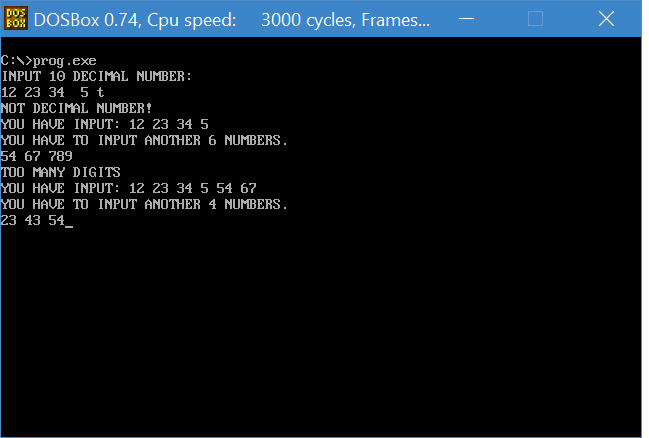
\includegraphics[width=\textwidth]{1.png}
\caption{输入过程(目前输入9个数字)}
\label{1}
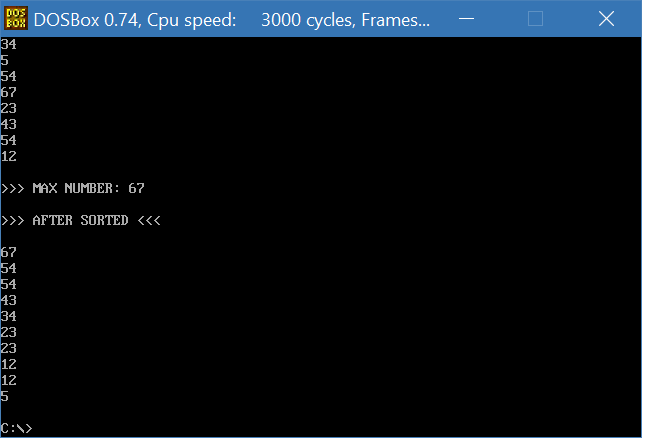
\includegraphics[width=\textwidth]{2.png}
\caption{输出和排序过程}
\label{2}
\end{figure}
\section{思考题}
\begin{enumerate}
\item 若处理的是十六进制无符号数,程序应如何修改?

在字符存取的部分修改即可,加上判断,若字符为0到9,代码不变,存取时分别加减30H;若字符为
A到F,存取时加减37H。
\item 若处理的是带符号数,程序又应作何修改?

首先需要判断“-” 符号,然后根据正负号决定是否将两位数取补码后存储。取数时根据最高位判断正
负,决定输出到显示屏时是否要加上符号,客观的说,处理带符号数的难度要上升很多
\end{enumerate}
\section{完成情况}
本次实验因为准备充分,代码的调试已经事先完成,因此效果较好,在本次实验中,我理解了条件转移职能进行近地址跳转而不能进行远地址跳转并且使用函数解决了问题。同时,在使用函数的过程中,尽可能的避免了栈上空间的操作(程序中没有栈上空间的操作,所有的操作除了对数据块的读取外均在寄存器上进行),从最大程度上节约了运行时间,尽管,设计合适的压栈和函数可以进一步增加代码的可读性,但是作为低级语言,相对语言本身更在意的就是程序的执行效率,因此为了提高运行效率,可读性的牺牲也是可以理解的,虽然作为题目中的数据规模,避免内存访问所带来的运行时间减少是微乎其微的,但是作为对编程能力的锻炼仍然有着很大的意义
\end{document}